
\section{A1}

\subsection{A1.1}

\subsubsection{a}

We need to identify all the sources of non-determinism in the model. 

At the guard create1 in the client module, there's non-determinism. The same applies to the guard create2.
\begin{verbatim}
// Create a new job - length chose non-deterministically
  [create1] state1=0 -> (state1'=1) & (task1'=1);
  [create1] state1=0 -> (state1'=1) & (task1'=2);
  [create1] state1=0 -> (state1'=1) & (task1'=3);
  [create1] state1=0 -> (state1'=1) & (task1'=4);
  [create1] state1=0 -> (state1'=1) & (task1'=5);
\end{verbatim}
This is due to local non-determinism because this doesn't depend on the concurrent execution of two modules.

In the module scheduler at the guard create1 and create2 there's non-determinism.
\begin{verbatim}
// Place a new job at the end of the queue
  [create1] job2=0 -> (job2'=1);
  [create2] job2=0 -> (job2'=2);
\end{verbatim}
This is due to the concurrent execution of two modules. Two actions are executed concurrently.

\subsubsection{b}
The local non-determinism is resolved by including probabilistic commands:
\begin{verbatim}
[create1] state1=0 -> 0.2 : (task1'=1) & (state1'=1) + 
0.2 : (task1'=2) & (state1'=1) + 0.2 : (task1'=3) & (state1'=1) + 
0.2 : (task1'=4) & (state1'=1) + 0.2 : (task1'=5) & (state1'=1);
\end{verbatim}
The uniform distribution is 0.2. The model can be seen in the appendix.

\subsubsection{c}
The model has 83 states.

\subsubsection{d}
They remain the same because they are different actions.

\subsubsection{e}
The qualitative PCTL formula holds for the model:
\begin{verbatim}
P=? [ (task1>0)=>(P>=1 [ F (task1=0) ]) ]
\end{verbatim}

\subsection{A1.2}

\subsubsection{a}

Using Model: Compute: Steady-state probabilities:

\begin{verbatim}
0:(0,0,0,0,0,0)=0.016145825133811565
1:(0,0,1,0,2,0)=0.016145821765883802
...
\end{verbatim}

The probability for no jobs in the queue is: $0.016145825133811565 = 1.6145825133811565\% \approx 1.61\%$
This can be read directly from the steady-state probability for $(0,0,0,0,0,0)$,
because $(0,0,0,0,0,0)$ is the only state in which job1 and job2 are zero,
or it can be computed in PRISM by "verifying" the property:

\begin{verbatim}
S=? [job1=0 & job2=0]
\end{verbatim}

\subsubsection{b}

We first find the steady-state probabilities for task1=0..5.
This could also be done by manually summing for each i in 0..5
the steady-state probabilities for the states where task1 = i.

\begin{verbatim}
p0 = S=? [task1=0] ~ 0.34140
p1 = S=? [task1=1] ~ 0.16776
p2 = S=? [task1=2] ~ 0.15057
p3 = S=? [task1=3] ~ 0.13286
p4 = S=? [task1=4] ~ 0.11411
p5 = S=? [task1=5] ~ 0.09328
\end{verbatim}

The expected length is then found by
multiplying the length with its steady-state probability:

$0*p0 + 1*p1 + 2*p2 + 3*p3 + 4*p4 + 5*p5 =$

$0.16776 + 2*0.15057 + 3*0.13286 + 4*0.11411 + 5*0.09328 =$

$1.79032$

\subsubsection{c}

The transient distribution for time t = 10 is computed by
selecting Model:Compute:"Transient probabilities"
and giving the argument 10:

\begin{verbatim}
0:(0,0,0,0,0,0)=0.0175
1:(0,0,1,0,2,0)=0.018750000000000003
...
\end{verbatim}

We sum up the probabilities for state1=0 in the transient state probabilities:
$0.0175 + 0.01875 + 0.008 + 0.04275 + 0.008 + 0.0415 + 0.008 + 0.039 + 0.008 + 0.034 + 0.008 + 0.024 =$

$0.2575$

The result fits with the "verification" of the property

\begin{verbatim}P=? [ X X X X X X X X X X state1=0]\end{verbatim},

which is written in PCTL*.

\subsubsection{d}

The probabilities are calculated using PCTL*.

\begin{verbatim}
1.0
0.5
0.5
0.25
0.15
0.1625
0.225
0.259375
0.283125
0.3125
0.2575
\end{verbatim}

\begin{figure}[!htb]
\centering
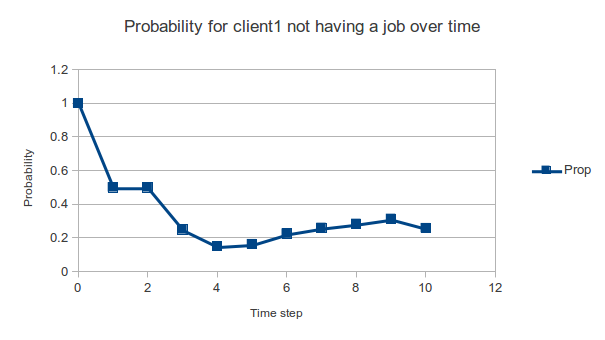
\includegraphics[scale=.75]{images/chart_client1_nojob_time_prop.png}
\caption{Probability for client one not having a job over discrete time}
\label{fig:nojobprop}
\end{figure}

In the start, the client does not have a job.
After that, the probability for not having a job falls a lot,
since it is likely that client 1 gets a job in immediately
or shortly after client 2 has gotten a job and has had its
job move into the first queue field.

After that, the probability rises, since client 1 could
have had its job in the queue, and it becomes likely that
its job is finished, thus meaning that it is not in the queue.

After that, the probability begins to oscillate towards 0.25,
since 0.25 is the steady-state probability of client 1 not having a job in the queue.

\subsection{A1.3}

\subsubsection{a}

\begin{verbatim}
P>0.2 [ X task1>2]
\end{verbatim}

Verified to be true.

\subsubsection{b}

\begin{verbatim}
P<0.5 [F<=10 task2=5]
\end{verbatim}

Verified to be true.

\subsubsection{c}

\begin{verbatim}
P>0 [G state1=1]
\end{verbatim}

Verified to be false.

\subsubsection{d}

\begin{verbatim}
P=? [ X task1>2] = 0.3
P=? [F<=10 task2=5] ~ 0.26209
P=? [G state1=1] = 0.0
\end{verbatim}

\subsection{A1.4}

\subsubsection{a}

$M$ is some discrete-time Markov chain (DTMC),
$\Phi$ is some CTL formula.

$T_M$ is the transition system obtained from the Markov chain
by the following definitions:

$S_{T_M} = S_M$

$Act_{T_M} = \{\tau\}$

$\to_{T_M} = \{(s_i, t, s_j) \in S_M \times Act_{T_M} \times S_M | P_M(i, j) > 0\}$

$I_{T_M} = \{s_i \in S_M | {\iota_{init}}_M(i) > 0\}$

$AP_{T_M} = AP_M$

$L_{T_M} = L_M$

We define a DTMC satisfying a CTL-formula as follows:

$M \models \Phi$ if $T_M \models \Phi$

\subsubsection{b}

Example:

$S = {s_0, s_1}$

$P(0, \_) = [0.5, 0.5]$

$P(1, \_) = [0.0, 1.0]$

$\iota_{init} = [1.0, 0.0]$

$AP = \{\Phi\}$

$L = \{s_0 \to \{\Phi\}, s_1 \to \{\}\}$

\subsubsection{c}

The formula clearly holds for $EG \Phi$,
since we start in $s_0$ and can stay there
forever.

The formula does not hold for $\neg P_{\leq 0} G \Phi \Leftrightarrow P_{>0} G \Phi$,
since staying in $s_0$ forever is the only
path where $\Phi$ holds forever,
and the probability of that path is 0.

\subsubsection{d}

Fairness, in the sense that paths that are extremely unlikely (and thus "unfair")
are excluded.
That way, the "unfair" path that stays in $s_0$ forever would be excluded from consideration.
CTL does not provide fairness, while fairness can be dealt with in LTL and CTL*.

